\section{Results and Interpretation}
\noindent The Principle Component Analysis (PCA) of our features are shown in Fig ~\ref{flippca} 

\begin{figure}[H]
\begin{center}
\includegraphics [width=0.5\textwidth]{flip_binary_feature_HOMO.png}
\caption{PCA}\label{flippca}
\end{center}
\end{figure}

We have plotted the test results versus different machine learning methods for various features in Fig ~\ref{homo}, Fig ~\ref{lumo} and Fig ~\ref{gap}. These results show that machine learning algorithms run well on our feature vectors and predict reasonable values for HOMO, LUMO, and band gap. In all figures, the prediction errors from other machine learning algorithms are well below the ``mean" method, indicating that these methods work better than random guess. For a certain algorithm, prediction errors from all features that we have developed are all significantly lower than null feature, which shows that our feature extraction also works better than just making predictions based on which dataset the structure came from. SVM and Decision Tree methods already show particularly low test errors and can be utilized for chemical calculation to some extent.

\begin{figure}[H]
\begin{center}
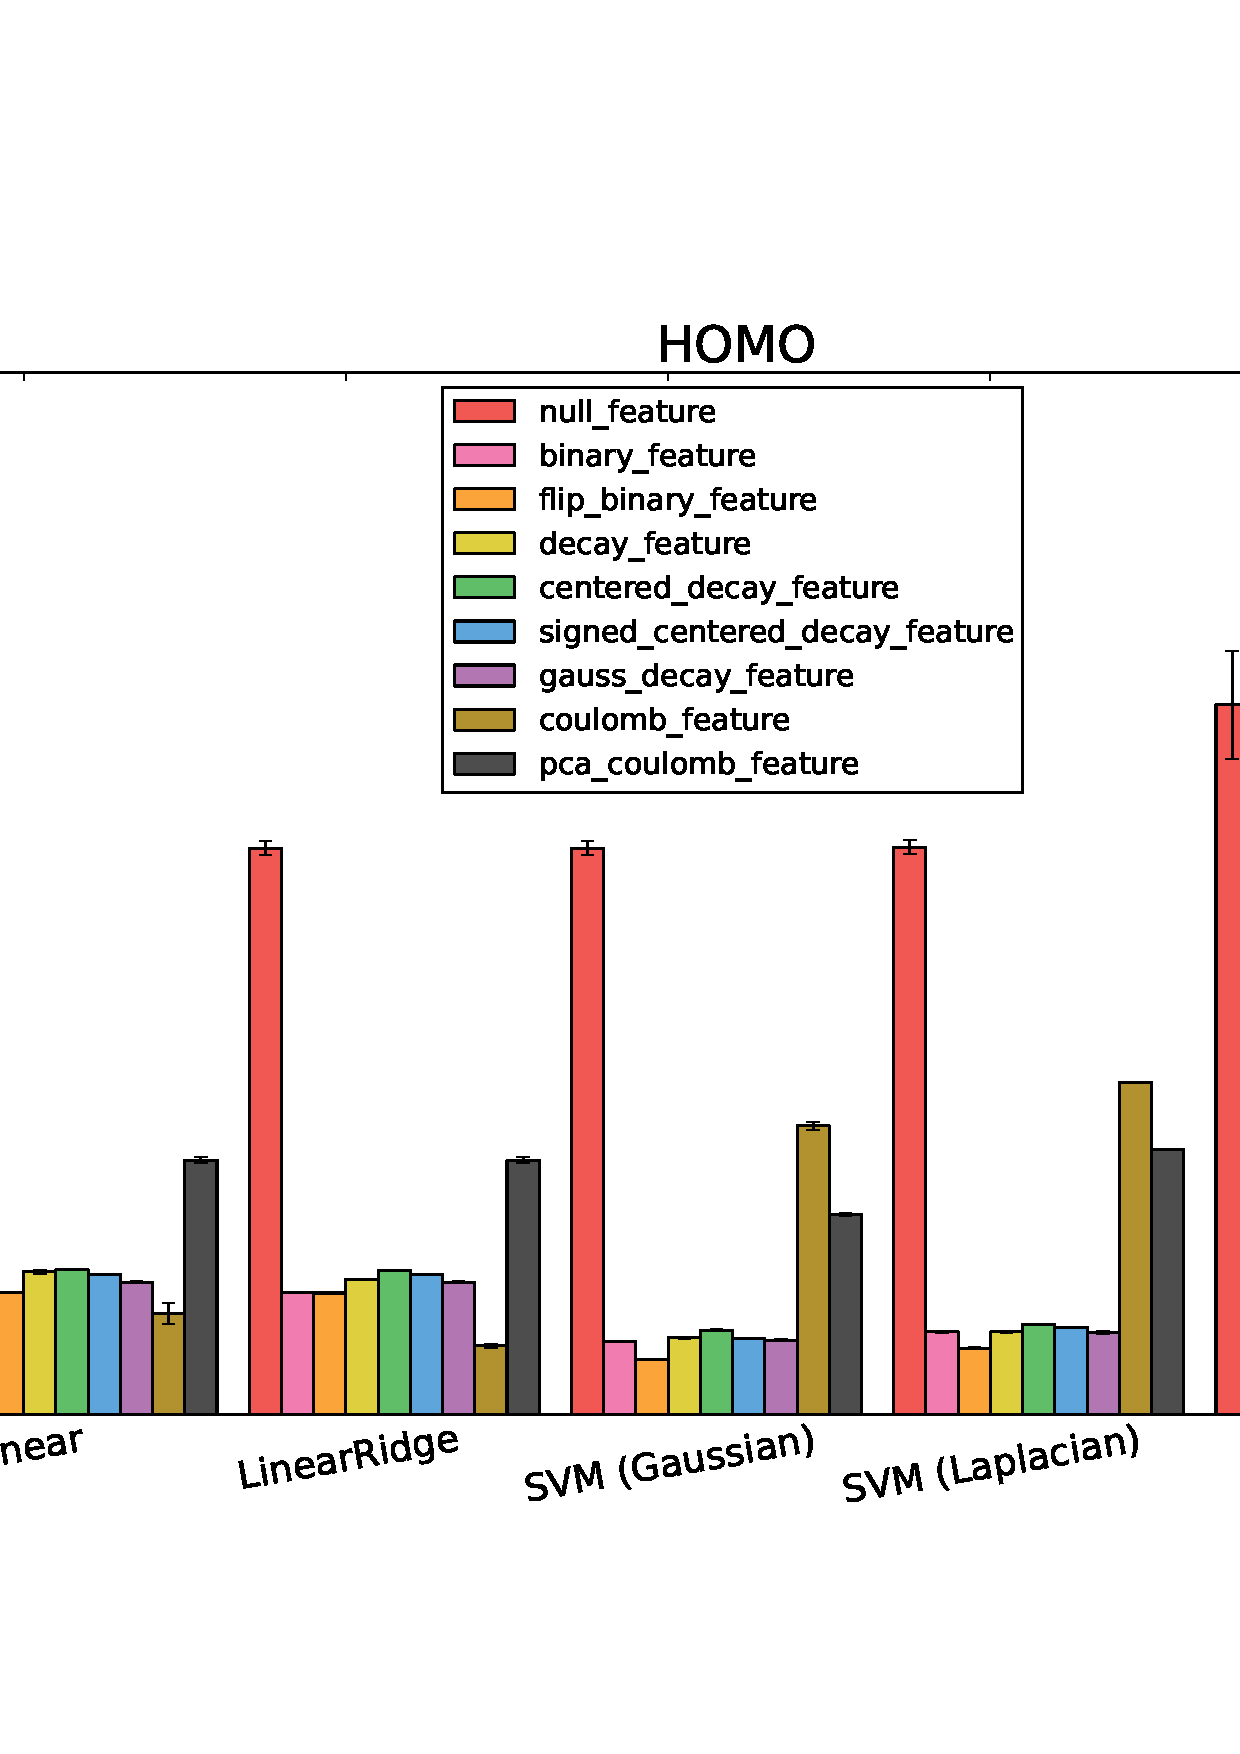
\includegraphics [width=1\textwidth]{homo_results.png}
\caption{test errors of HOMO}\label{homo}
\end{center}
\end{figure}

\begin{figure}[H]
\begin{center}
\includegraphics [width=1\textwidth]{lumo_results.png}
\caption{test errors of LUMO}\label{lumo}
\end{center}
\end{figure}

\begin{figure}[H]
\begin{center}
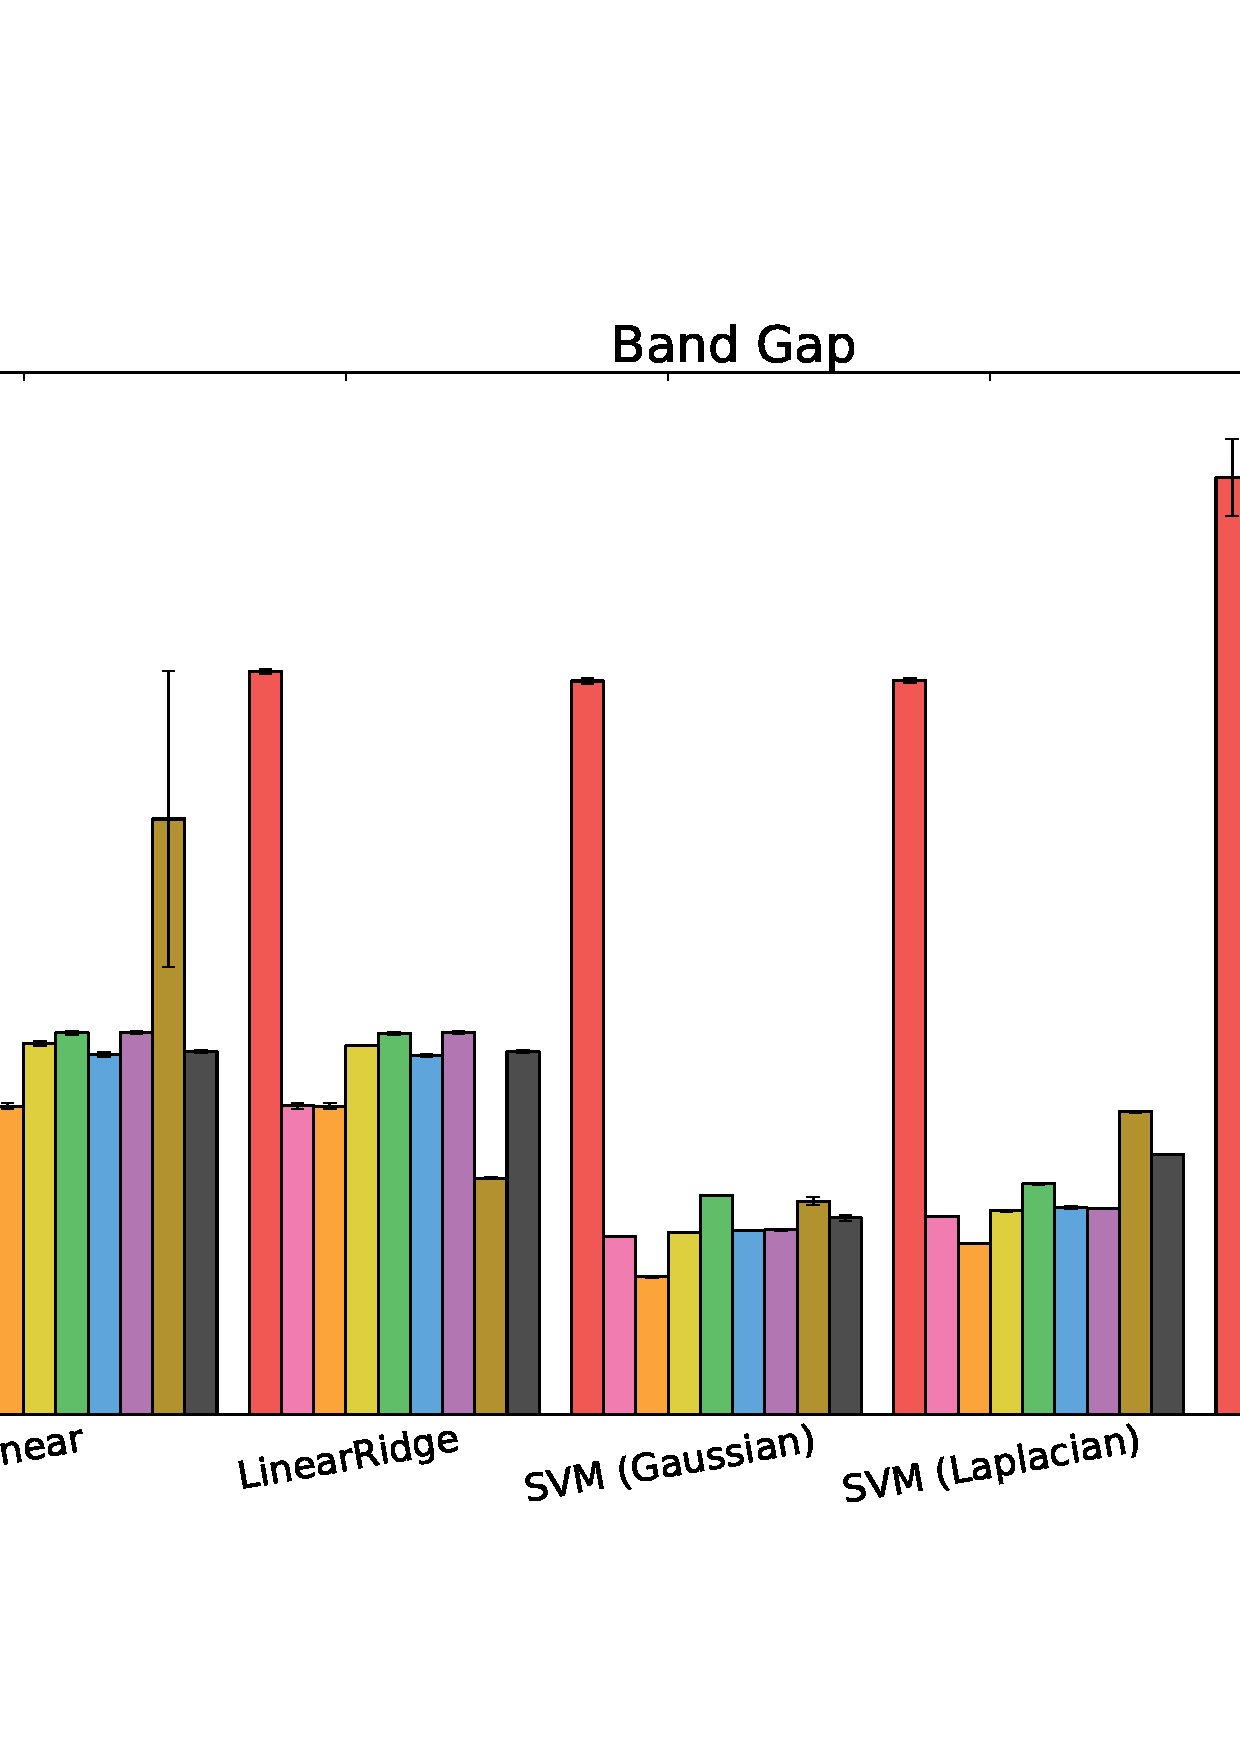
\includegraphics [width=1\textwidth]{gap_results.png}
\caption{test errors of band gap}\label{gap}
\end{center}
\end{figure}
Overall, the flip binary feature vector has the best performance of all the feature vectors. This can be attributed to two factors, 1) it contains more relevant information than the binary feature, so it will quite readily out perform it. 2) This implies that the decay function used in the decay feature vectors is not a good representation of the physical relation between the structures.

To further lower the test errors, we apply Neural Networks with sigmoid or tanh layers to our dataset. Neural Networks' PCA and predictions have shown ideal results in Fig ~\ref{nnpca} and  (Neural INDO comparison plots). Gradient evolution in PCA plots indicates that each layer of the networks can assign the prediction values effectively. 

\begin{figure}[H]
\begin{center}
\includegraphics [width=0.6\textwidth]{07_conn.png}
\caption{Neural Networks PCA}\label{nnpca}
\end{center}
\end{figure}

Neural Networks produce 0.55, 0.60, 0.72 kcal/mol errors for HOMO, LUMO, and Band Gap respectively, which are much lower than the chemical accuracy 1 kcal/mol. 
